\subsection{\name in Testbed Experiments}
\label{sec:testbed}

\subsubsection{BPF in practice}

\begin{figure}[!t]
    \centering
    
\includegraphics[width=0.3\linewidth]{fig/b1_mov_legend} 
    \\
    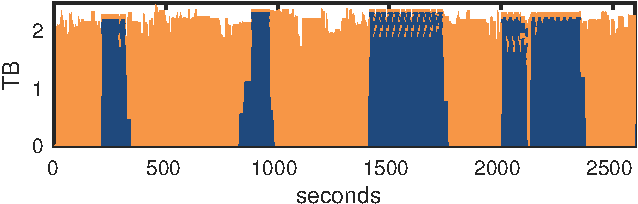
\includegraphics[width=0.8\linewidth]{fig/b1_mov_SpeedFair_BB} 
    \caption{[Cluster] \name's solution for the motivational problem (\S\ref{sec:ex}). The first two jobs of {\burstq} quickly finish and the last two jobs are prevented from using too much resource. This solution is close to the optimal one.}
    \label{fig:solution}
\end{figure}

Before diving into the details of our evaluation, recall the motivational problem from Section~\ref{sec:ex}. 
Figure~\ref{fig:solution} depicts how \name solves it in the testbed. \name enables the first two jobs of {\burstq} to quickly finish in 141 and 180 seconds.
For the two large jobs arriving at 1400 and 2000 seconds, the share is very large only in roughly 335 seconds but it is cut down to give back resource to {\batchq}.
%The large job arrives at 1400 seconds is not continuously allocated with large resources like SP.

\subsubsection{Performance guarantee}
\label{sec:performane_guarantee}

\begin{figure}[!t]
\centering
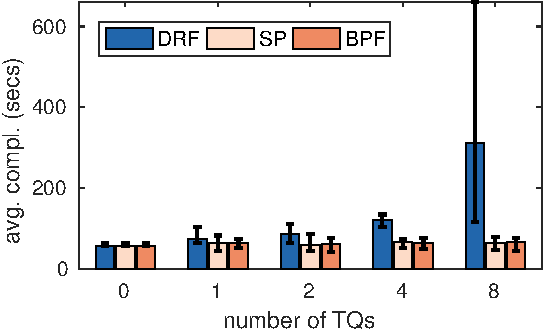
\includegraphics[width=0.8\linewidth]{fig/busty_perf_grt_err_BB}
\caption{[Cluster] Average completion time of \burstq jobs in a single \burstq across the 3 schedulers when varying the number of {\batchq}s. \name and SP guarantee the average completion time of the \burstq jobs while DRF significantly suffers from the increase of number of {\batchq}s.}
\label{fig:busty_perf_grt}
\end{figure}
 
Next, we focus on what happens when there are more than one \batchq.
Figure \ref{fig:busty_perf_grt} shows that average completion time of \burstq jobs in the 40-node cluster on the BB workload. In this setting, there are a single \burstq and multiple {\batchq}s. The x-axis shows the number of TQs in the cluster.

When there are no TQs, the average completion times of \burstq jobs across three schedulers are the same (57 seconds).
The completion times are greater than the average ON period (27 seconds) because of inefficient resource packing and allocation overheads.
In practice, the resource demand of tasks cannot utilize all resources of a node that results in large unallocated resources across multiple nodes.
Hence, the \burstq jobs are not able to receive the whole cluster capacity as expected.
More importantly, this delay is also caused by allocation overheads, such as waiting for containers to be allocated or launching containers.

As the number of {\batchq}s increases, the performance of DRF significantly degrades because DRF tends to allocate less resource to {\burstq} jobs.
DRF is the worst among three schedulers. In contrast, \name and SP give the highest priority to {\burstq}s that guarantees the performance of \burstq jobs.
The average completion times, when TQs are available (1,2,4, and 8), are almost the same (65 seconds).
These average completion times are still larger than the case of no TQs because of non-preemption.
The \burstq jobs are not able to receive the resources that are still used by the running tasks. 

\begin{table}[!t]
\centering
\caption{[Cluster] Factor of improvement by \name across various workload with respect to the number of {\batchq}s.} 
\begin{tabular}{|c|c|c|c|c|} \hline
\small
\centering
Workload & 1 TQ  & 2 TQs & 4 TQs & 8 TQs \\ \hline \hline
BB & 1.18 & 1.42 & 1.86 & 4.66 \\ \hline 
TPC-DS &  1.35 &   1.61  &  2.29  &  5.38  \\ \hline 
TPC-H & 1.10  & 1.37 & 2.01 &  5.12\\ \hline 
\end{tabular}
\label{tbl:speed_up}
\end{table}

To understand how well \name performs on various workload traces, we carried out the same experiments on TPC-DS and TPC-H.
As SP and \name achieve the similar performance, we only present the factors of improvement of \name across the various workloads in Table \ref{tbl:speed_up}.
The numbers on the table show the consistent improvement on the average completion time of \burstq jobs. 

\begin{figure}[!t]
    \centering
    \subfloat[1 LQ \& 4 TQs]{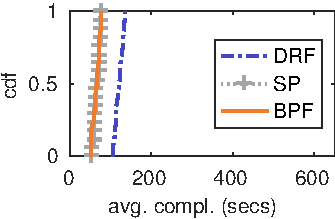
\includegraphics[width=0.48\linewidth]{fig/busty_perf_grt_cdf4_BB} \label{fig:busty_perf_grt_cdf_a}}    
    \subfloat[1 LQ \& 8 TQs]{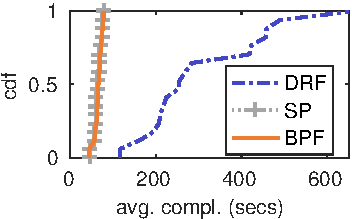
\includegraphics[width=0.48\linewidth]{fig/busty_perf_grt_cdf8_BB} \label{fig:busty_perf_grt_cdf_b}}
    \caption{[Cluster] The completion time of LQ jobs is predictable using \name.}
    \label{fig:busty_perf_grt_cdf}
    \vspace{-0.4cm}
\end{figure}

In addition to the average completion time, we evaluated the performance of individual \burstq jobs.
Figure \ref{fig:busty_perf_grt_cdf} shows that cumulative distribution functions (cdf) of the completion times across 3 approaches.
Figure \ref{fig:busty_perf_grt_cdf_a} and \ref{fig:busty_perf_grt_cdf_b} are the experimental results for the cases of 4 {\batchq}s and 8 {\batchq}s, respectively.
We observe that the completion times of \burstq jobs in DRF are not stable and vary a lot when the number of {\burstq}s becomes large as in Figure \ref{fig:busty_perf_grt_cdf_b}.
The unstable performance is caused by the instantaneous fairness and the variance of total resource demand.

\subsubsection{Fairness guarantee}
\label{sec:fairness_guarantee}

\begin{figure}[!t]
    \centering
    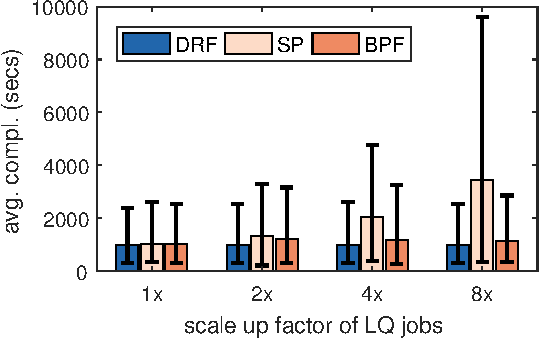
\includegraphics[width=0.8\linewidth]{fig/batch_perf_protect_BB} 
%    \\
%    \subfloat[LQ jobs]{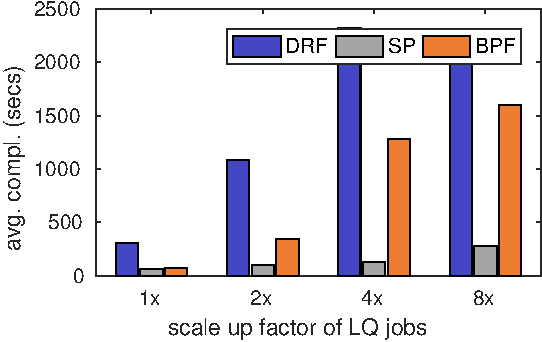
\includegraphics[width=1\linewidth]{fig/long_busty_BB} \label{fig:protecting_batch_jobs_b}}
    \caption{[Cluster] \name protects the batch jobs up to $3.05\times$ compared to SP.}
    \vspace{-0.3cm}
    \label{fig:protecting_batch_jobs}
\end{figure}

Figure \ref{fig:protecting_batch_jobs} shows the average completion time of \batchq jobs when we scale up the number of tasks of \burstq jobs are by 1x, 2x, 4x, and 8x.
In this experiment, there are a single \burstq and 8 {\batchq}s.

Since DRF is a fair scheduler, the average completion times of \batchq jobs are almost not affected by the size of \burstq jobs.
However, SP allocates too much resource to \burstq jobs that significantly hurts \batchq jobs.
Since SP provides the highest priority for the {\burstq} jobs, it makes the {\batchq} jobs to starve for resources.
\name performs closely to DRF.
While DRF maintains instantaneous fairness, \name maintains the long-term fairness among the queues.


%\begin{figure}[!t]
%\centering
%    {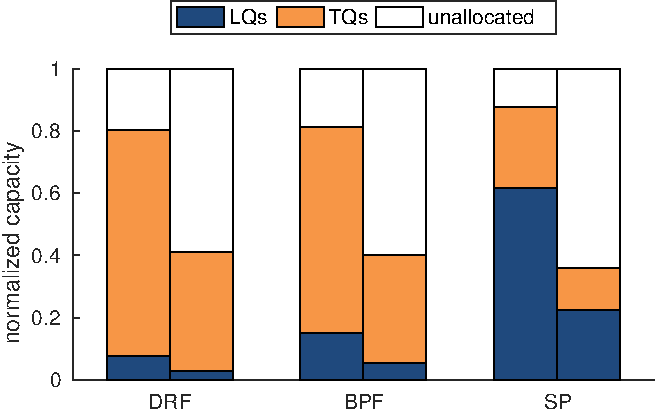
\includegraphics[width=0.8\linewidth]{fig/b8_avg_res_BB}}
%\caption{[Cluster] The average resource consumption of the cases of scaling up \burstq jobs at 8x. The left bar is memory usage, and the right bar is CPU usage. All three policies have similar utilization.}
%\label{fig:avg_res}
%\end{figure}

%To better see the long-term fairness in resource allocation, we present average resource usage across 3 approaches in Figure \ref{fig:avg_res}.
%There are totally 9 queues (1 \burstq and 8 \batchq). The x-axis is the normalized capacity.
%SP is dominant in both memory and CPU.
%\name and DRF can achieve the fairness in resource allocation for {\burstq}s and {\batchq}s.
%All of them have similar resource utilization.

\subsubsection{Scheduling overheads}

Recall from Section \ref{sec:impl} that the \name scheduler has three components: user input, admission control, and allocation.
Compared to the default schedulers in YARN, our scheduler has additional scheduling overheads for admission control and additional computation in allocation.

Since we only implement our scheduler in the Resource Manager, the scheduling overheads occur at the master node.
To measure the scheduling overheads, we run admission control for 10000 \burstq queues and 10000 \batchq queues on a master node -- Intel Xeon E3 2.4 GHz (with 12 cores).
Each LQ queue has 500 ON/OFF cycles.
Recall the \textsc{LQAdmit} and \textsc{TQAdmit} functions in Algorithm \ref{algorithm1}, the admission overheads increase linearly to the number of queues.
The total admission overheads are approximately 1 ms, which is much less than the default update interval in YARN Fair Scheduler, i.e., 500 ms \cite{hadoop-fair-scheduler}.
The additional computation in allocation is also negligibly less than 1 ms.

%\begin{table*}
%\centering
%\caption{Scheduling overheads} 
%\begin{tabular}{|c|p{10cm}|c|} \hline
%Type & Description & Avg. Time \\ \hline \hline
%Job submission & Job is submitted from client to YARN & 13.22 secs \\ \hline
%Container allocation & YARN localizes and allocates a container for a task.  &  0.04 secs \\ \hline
%Task setup & Tez setup a task to run on the allocated container. & 6.24 secs \\ \hline
%Launching Tez task & Launching a Tez task on the container & 1.17 secs \\ \hline
%Task stop & Tez stops the container use on a finished task. & 0.21 secs\\ \hline
%Container release & YARN releases the running container. & 5.19 secs \\ \hline
%\end{tabular}
%\label{tbl:schedulingOverheads}
%\end{table*}

\subsubsection{Admission control for multiple LQs}
\label{sec:admission}

\begin{figure}[!h]
	\centering
	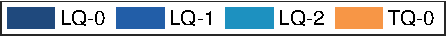
\includegraphics[width=0.6\linewidth]{fig/b1i3_res_usage_legend} 
	\vspace{-0.1cm}
	\subfloat[DRF: \burstq-0, \burstq-1, \burstq-2 are unhappy with high latency.]{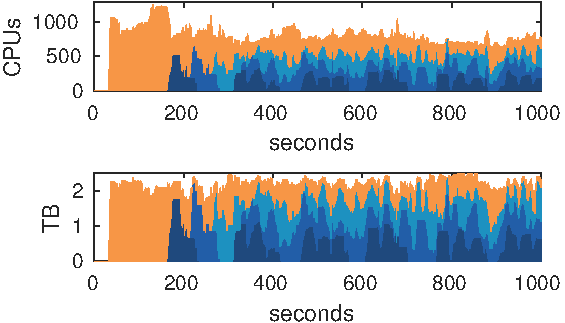
\includegraphics[width=0.8\linewidth]{fig/res_usage_b1i3_DRF_BB} \label{fig:admission_drf_cluster}} 

	\subfloat[SP: \batchq-0 is starving of resources.]{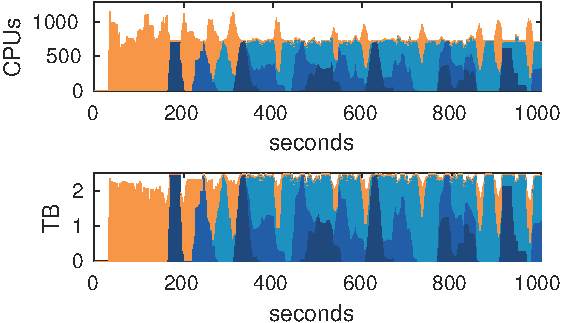
\includegraphics[width=0.8\linewidth]{fig/res_usage_b1i3_SP_BB} \label{fig:admission_strict_cluster}}
    
	\subfloat[N-\name: Only {\burstq}-0 and {\batchq}-0 are happy.]{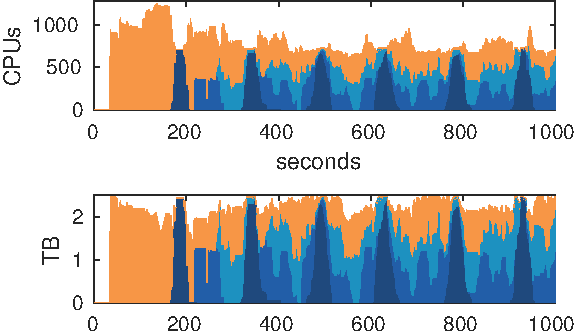
\includegraphics[width=0.8\linewidth]{fig/res_usage_b1i3_N-BPF_BB} \label{fig:admission_hard_cluster}}
   
	\subfloat[\name: {\burstq}-0, {\burstq}-1 and {\batchq}-1 are happy.]{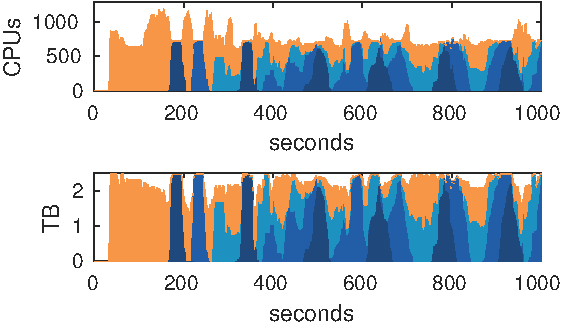
\includegraphics[width=0.8\linewidth]{fig/res_usage_b1i3_BPF_BB} \label{fig:admission_speedfair_cluster}}

	\caption{[Cluster]. DRF and SP fail to guarantee both performance and fairness simultaneously. \name gives the best performance to \burstq-0, near optimal performance for \burstq-1, and maintains fairness among 4 queues. \burstq-2 requires too much resource, so its performance cannot be guaranteed.}
	\label{fig:admission_control_cluster}
\end{figure}


To demonstrate how \name works with multiple {\burstq}s, we set up 3 {\burstq}s (\burstq-0, \burstq-1, and \burstq-2) and a single \batchq (TQ-0).
The jobs \batchq-0 are queued up at the beginning while \burstq-0, \burstq-1, and \burstq-2 arrive at 50, 100, and 150 seconds, respectively.
The periods of {\burstq}-0, {\burstq}-1, and {\burstq}-2 are 150, 110, and 60 secs. All the {\burstq}s jobs have the identical demand and task durations.
The TQ jobs are chosen from the BB benchmark.
\name admits {\burstq}-0 to the Hard Guarantee class, {\burstq}-1 to the Soft Guarantee class, and {\burstq}-2 to the Elastic class.

Figure \ref{fig:admission_drf_cluster} shows the resource usage (CPU and memory) for each queue across four schedulers, i.e., DRF, SP, N-\name and \name.
As an instantaneously fair scheduler, DRF continuously maintains the fair share for all queues as in Figure \ref{fig:admission_drf_cluster}.
Since \burstq-2 requires a lot of resources, SP makes \batchq-0 starving for resources (Figure \ref{fig:admission_strict_cluster}). N-\name provides \burstq-0 with resource guarantee and it fairly share the resources to \burstq-1, \burstq-2, and \batchq-0 (Figure \ref{fig:admission_hard_cluster}).
\name provides hard guarantee to \burstq-0 and soft guarantee to \burstq-1 as in Figure \ref{fig:admission_speedfair_cluster}.
The soft guarantee allows \burstq-1 performs better than using N-\name.
Since \burstq-2 demands too much resources, \name treats it like \batchq-0.

Figure \ref{fig:avg_multi_queue_cluster} shows the average completion time of jobs on each queue across the four schedulers.
The performance of DRF for \burstq jobs is the worst among the four schedulers but it is the best for only \batchq-0.
The performance of SP is good for \burstq jobs but it is the worst for \batchq jobs.
N-\name provides the best performance for \burstq-0 but not \burstq-1 and \burstq-2.
\name is the best among the four schedulers.
The three of four queues, i.e., \burstq-0, \burstq-1, and \batchq-0, significantly benefit from \name.
\name even outperforms SP for \burstq-0 and \burstq-1 jobs and does not hurt any {\batchq}.

\begin{figure}[!h]
	\centering
	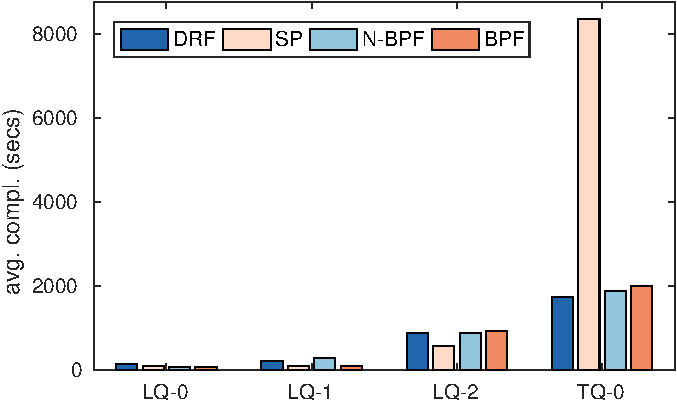
\includegraphics[width=0.8\linewidth]{fig/avg_multi_queues_impl}
	\caption{[Cluster] \name provides with better performance for {\burstq}s than DRF and N-\name. Unlike SP, \name protects the performance of \batchq jobs.}
	\label{fig:avg_multi_queue_cluster}
\end{figure}
